\chapter{Planificación, metodología y presupuesto}

\section{Metodología de desarrollo}

\subsection{Paradigma ágil}

El desarrollo de software conlleva una complejidad intrínseca que requiere de metodologías de gestión capaces de adaptarse a entornos cambiantes. Históricamente, los enfoques predictivos o tradicionales se han basado en una planificación exhaustiva y un control riguroso del ciclo de vida, definiendo de manera estricta las actividades, los artefactos y los roles desde el inicio del proyecto. Si bien este modelo ha demostrado su eficacia en proyectos con requisitos estables y predecibles, presenta limitaciones significativas cuando las especificaciones evolucionan durante el desarrollo.

Frente a este paradigma surge la filosofía ágil, que desplaza el centro de gravedad del proceso desde el cumplimiento rígido del plan hacia la entrega continua de valor y la colaboración con los \textit{stakeholders}. Sus fundamentos se articularon en el Manifiesto Ágil \cite{canos2003metodologias}, que establece cuatro valores esenciales: los individuos y las interacciones sobre los procesos y las herramientas, el software funcional sobre la documentación exhaustiva, la colaboración con el cliente sobre la negociación contractual, y la respuesta ante el cambio sobre el seguimiento de un plan.

\subsection{Scrum como marco de trabajo}

Dentro del paradigma ágil, Scrum constituye el marco de trabajo más ampliamente adoptado en la industria del software. Scrum no es una metodología prescriptiva, sino un contenedor ligero que define una estructura de roles, eventos y artefactos sobre la que se integran prácticas específicas de ingeniería. Su fundamento teórico descansa en el empirismo: el conocimiento proviene de la experiencia y las decisiones se basan en lo observado. Esto se materializa en tres pilares: la transparencia, que garantiza que el proceso y el trabajo sean visibles para todos los implicados; la inspección, que permite revisar el progreso con frecuencia para detectar desviaciones; y la adaptación, que ajusta el proceso cuando se identifica una desviación.

\subsubsection{Roles}

El equipo Scrum se compone de tres roles con responsabilidades bien definidas:

\begin{itemize}
    \item \textbf{Product Owner:} Responsable de maximizar el valor del producto. Gestiona el \textit{Product Backlog}, prioriza los requisitos y comunica el objetivo del producto al equipo.
    \item \textbf{Scrum Master:} Facilita la aplicación de Scrum dentro del equipo. Elimina impedimentos, asegura que se sigan las prácticas del marco y protege al equipo de distracciones externas.
    \item \textbf{Developers:} Profesionales que realizan el trabajo de construcción del producto. Se autoorganizan para entregar el Incremento en cada Sprint.
\end{itemize}

\subsubsection{Eventos}

Scrum define cinco eventos con duración fija, también llamados eventos time-boxed, que establecen la cadencia del trabajo:

\begin{itemize}
    \item \textbf{Sprint:} Iteración de duración fija, generalmente de entre una y cuatro semanas, durante la cual se construye un Incremento de producto potencialmente entregable.
    \item \textbf{Sprint Planning:} Reunión al inicio del Sprint donde el equipo acuerda el Objetivo del Sprint y selecciona los elementos del \textit{Product Backlog} que se abordarán.
    \item \textbf{Daily Scrum:} Reunión diaria de 15 minutos donde los desarrolladores sincronizan el trabajo y ajustan el plan para las próximas 24 horas.
    \item \textbf{Sprint Review:} Sesión al final del Sprint donde se presenta el Incremento a los \textit{stakeholders} y se recoge \textit{feedback} para ajustar las prioridades.
    \item \textbf{Sprint Retrospective:} Último evento del Sprint, donde el equipo inspecciona su propio proceso e identifica mejoras para aplicar en el siguiente ciclo.
\end{itemize}

\subsubsection{Artefactos}

Los artefactos de Scrum maximizan la transparencia de la información clave:

\begin{itemize}
    \item \textbf{Product Backlog:} Lista ordenada y emergente de todo lo que se sabe que es necesario para el producto. Es dinámica y evoluciona con el proyecto.
    \item \textbf{Sprint Backlog:} Conjunto de elementos del \textit{Product Backlog} seleccionados para el Sprint, más el plan para entregarlos y alcanzar el Objetivo del Sprint.
    \item \textbf{Incremento:} Suma de todos los elementos completados durante un Sprint y los anteriores. Cada Incremento debe cumplir con la \textit{Definition of Done} acordada por el equipo.
\end{itemize}

\subsection{Aplicación de Scrum al proyecto ReMind}

Dada la naturaleza del proyecto un desarrollo software de carácter individual con supervisión académica, se adoptó una adaptación de Scrum ajustada a sus particularidades. El equipo estuvo compuesto por el alumno como único desarrollador, encargado de la totalidad de la implementación, y el tutor académico, quien ejerció las funciones de \textit{Product Owner}, encargado de definir los requisitos, priorizar las funcionalidades y validar los resultados, y de \textit{Scrum Master}, responsable de supervisar el progreso, resolver impedimentos y asegurar la correcta aplicación del marco de trabajo. Al tratarse de un equipo unipersonal, el evento \textit{Daily Scrum} se sustituyó por una gestión autónoma del trabajo basada en la planificación semanal. En su lugar, las reuniones de sincronización y revisión se materializaron en sesiones quincenales con el tutor, donde se presentaban los incrementos completados durante la Sprint Review, se recogía feedback y se ajustaban las prioridades del siguiente ciclo en la Sprint Retrospective. Este formato permitió mantener los pilares de inspección y adaptación sin la sobrecarga de reuniones diarias innecesarias.

La planificación del proyecto se estructuró en seis \textit{Sprints} de duración variable, cada uno con un objetivo concreto que entregaba un Incremento funcional del producto:

\begin{itemize}
    \item \textbf{Sprint 0 -- Análisis y preparación, de 3 semanas de duración:} Investigación sobre la enfermedad de Alzheimer y las técnicas de estimulación cognitiva. Definición de requisitos funcionales y no funcionales. Estudio de las tecnologías disponibles y selección de la pila tecnológica.
    \item \textbf{Sprint 1 -- Diseño y prototipado, de 3 semanas de duración:} Elaboración del diseño arquitectónico del sistema, que incluye el diagrama de clases, el modelo de datos y el diseño de la API REST. Creación de \textit{mockups} de la interfaz de usuario. Configuración del entorno de desarrollo y del repositorio de código.
    \item \textbf{Sprint 2 -- Backend y autenticación, de 3 semanas de duración:} Implementación de la capa de persistencia mediante entidades JPA y repositorios. Desarrollo del sistema de autenticación y autorización basado en JWT y Spring Security. Creación de los controladores REST para la gestión de usuarios y agendas.
    \item \textbf{Sprint 3 -- Frontend y módulos básicos, de 4 semanas de duración:} Desarrollo de la estructura de componentes en Angular, que comprende la pantalla de inicio, la \textit{landing page} y el login. Implementación de los servicios de comunicación con la API. Creación de las vistas de gestión de pacientes y terapeutas.
    \item \textbf{Sprint 4 -- Desarrollo de los minijuegos, de 5 semanas de duración:} Implementación de los seis minijuegos cognitivos: ordenar secuencia, relacionar objetos, pagos exactos, vístete, completar oración e intruso. Desarrollo del sistema de niveles y dificultad progresiva.
    \item \textbf{Sprint 5 -- Integración, pruebas y despliegue, de 3 semanas de duración:} Integración completa de todos los módulos. Pruebas unitarias con JUnit y Mockito. Pruebas de integración de la API con Postman. Corrección de errores y elaboración de la documentación del proyecto.
\end{itemize}

\begin{figure}[H]
    \centering
    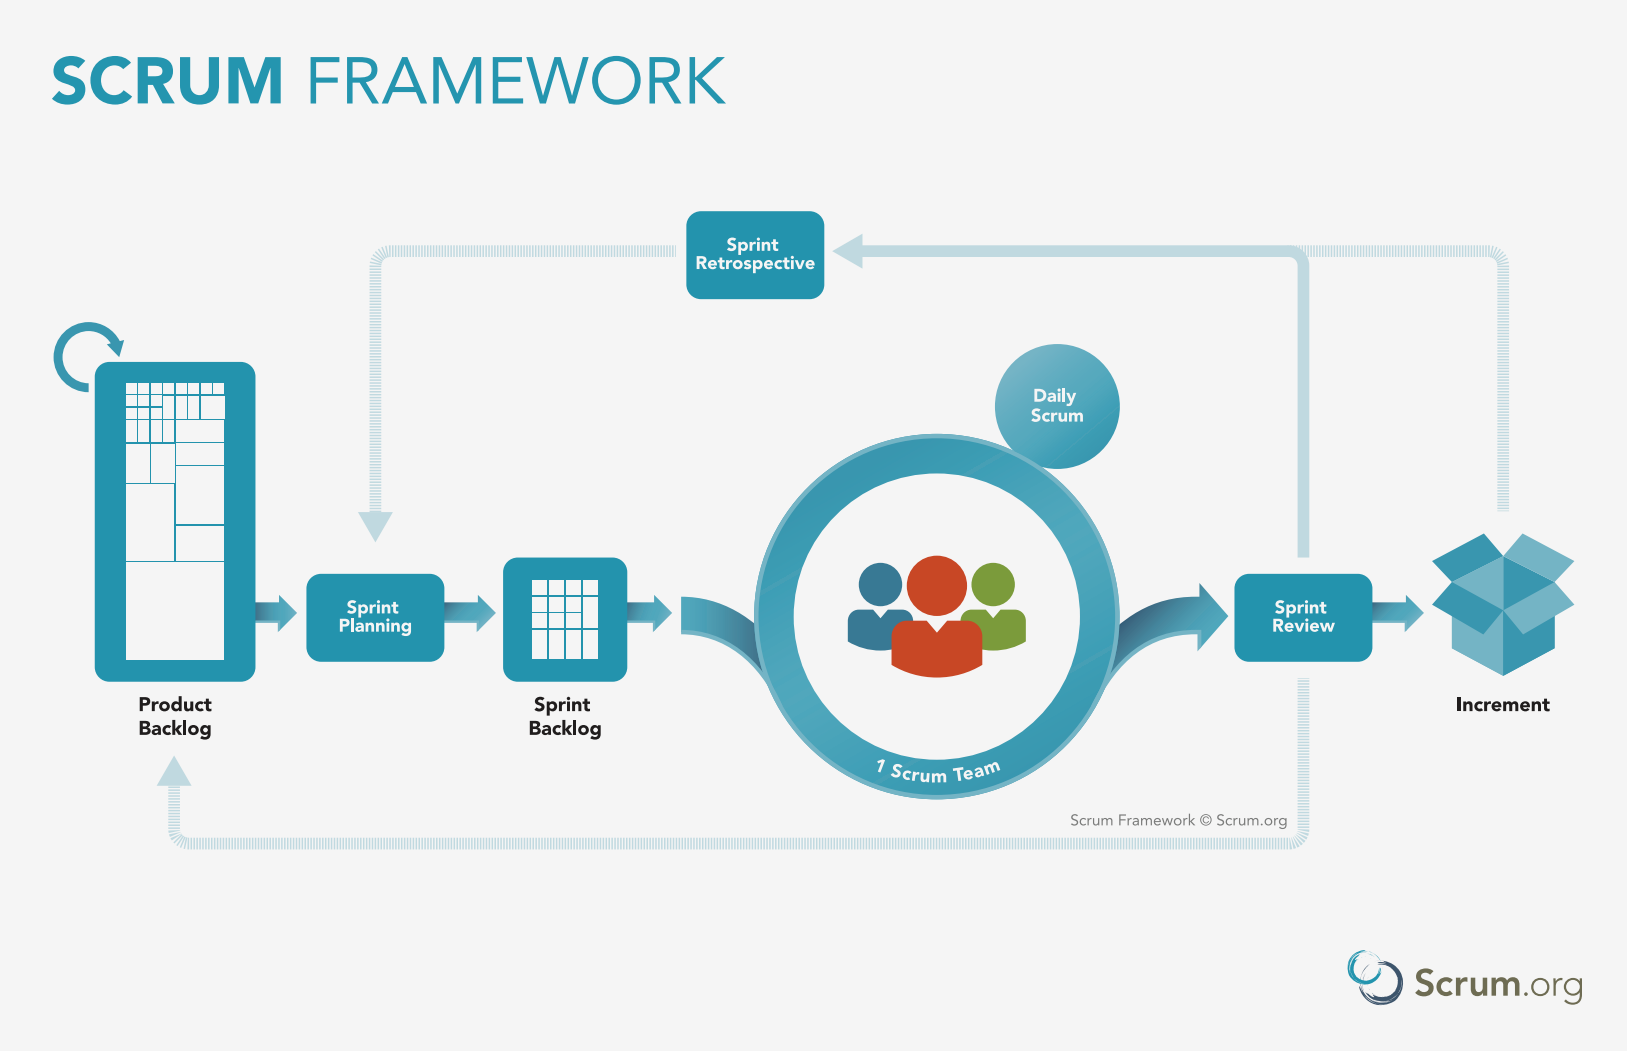
\includegraphics[width=0.7\textwidth]{imagenes/cronologia/scrum2.png}
    \caption{Esquema del proceso Scrum adaptado al proyecto ReMind.}
\end{figure}

\section{Planificación temporal}

La planificación temporal del proyecto se realizó utilizando una hoja de cálculo de Google Sheets, representando las tareas mediante un diagrama de Gantt que permite visualizar la secuencia y duración de cada actividad a lo largo del tiempo.

\begin{figure}[H]
    \centering
    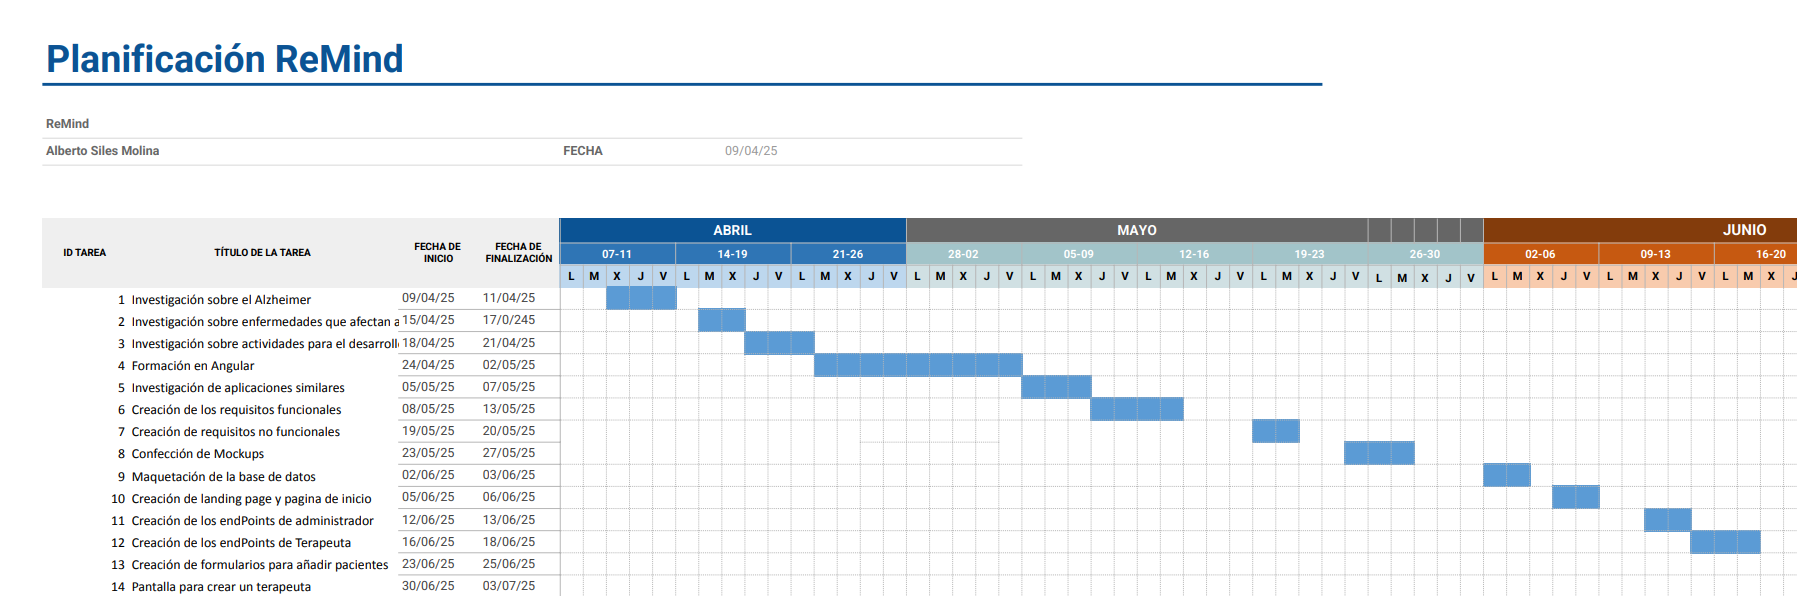
\includegraphics[width=\textwidth]{imagenes/cronologia/diagrama1.png}
    \caption{Diagrama de Gantt de la planificación temporal (1).}
    \label{fig:diagrama1}
\end{figure}

\begin{figure}[H]
    \centering
    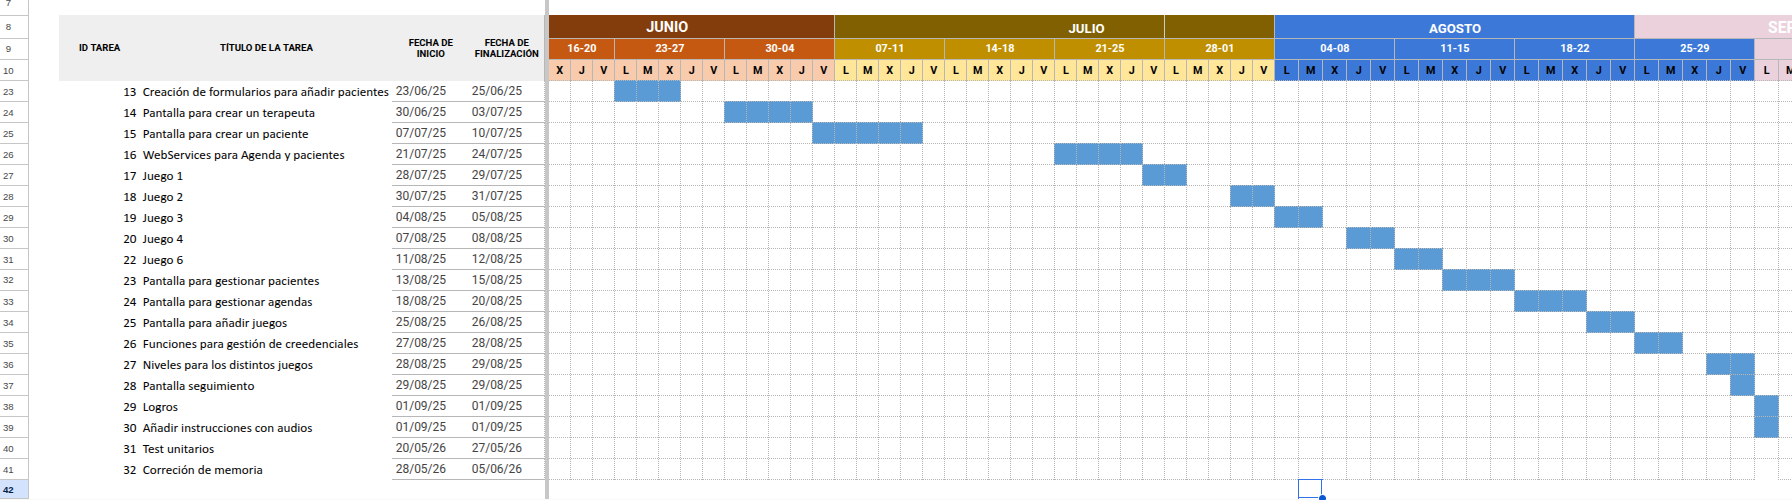
\includegraphics[width=\textwidth]{imagenes/cronologia/diagramaa2.png}
    \caption{Diagrama de Gantt de la planificación temporal (2).}
    \label{fig:diagrama2}
\end{figure}

\begin{figure}[H]
    \centering
    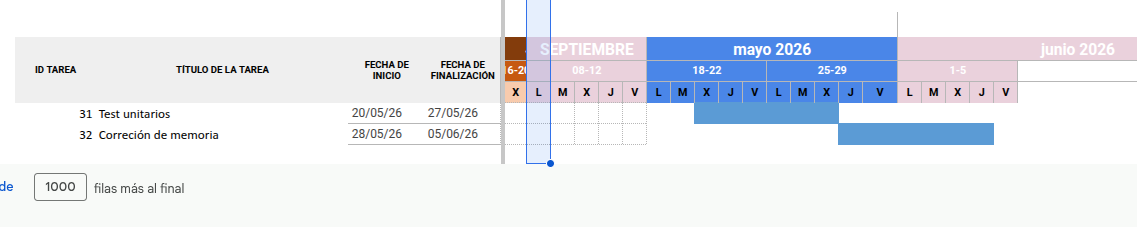
\includegraphics[width=\textwidth]{imagenes/cronologia/diagrama3.png}
    \caption{Diagrama de Gantt de la planificación temporal (3).}
    \label{fig:diagrama3}
\end{figure}

Cada recuadro del diagrama representa un bloque de 5 horas de trabajo, sumando un total de 370 horas planificadas para el proyecto. Las tareas se distribuyeron de manera progresiva, solapando ligeramente algunas actividades para optimizar los tiempos de desarrollo y permitir la integración temprana de componentes.

\begin{table}[H]
\centering
\caption{Distribución temporal por Sprint.}
\label{tab:sprints}
\begin{tabularx}{\textwidth}{|X|c|c|}
\hline
\textbf{Sprint} & \textbf{Duración} & \textbf{Horas estimadas} \\ \hline
Sprint 0 -- Análisis y preparación & 3 semanas & 45 h \\ \hline
Sprint 1 -- Diseño y prototipado & 3 semanas & 45 h \\ \hline
Sprint 2 -- Backend y autenticación & 3 semanas & 60 h \\ \hline
Sprint 3 -- Frontend y módulos básicos & 4 semanas & 70 h \\ \hline
Sprint 4 -- Desarrollo de minijuegos & 5 semanas & 100 h \\ \hline
Sprint 5 -- Integración, pruebas y documentación & 3 semanas & 50 h \\ \hline
\textbf{Total} & \textbf{21 semanas} & \textbf{370 h} \\ \hline
\end{tabularx}
\end{table}

\section{Planificación de costes}

A continuación se detallan los recursos necesarios para el desarrollo del proyecto y su coste asociado. Al tratarse de un Trabajo Fin de Grado de carácter académico y desarrollo individual, no se han considerado costes de personal contratado.

\begin{itemize}
    \item \textbf{Formación:} Se realizó un curso online sobre desarrollo web con Angular y Spring Boot, con un coste de 20 €.
    \item \textbf{Software y herramientas:} Se emplearon herramientas de desarrollo gratuitas o de código abierto: VSCode, Git, MySQL Community Edition, frameworks Spring Boot y Angular, entre otras.
    \item \textbf{Infraestructura:} El proyecto se desarrolló utilizando recursos locales, sin incurrir en costes de servidores o servicios cloud adicionales.
    \item \textbf{Equipo informático:} Se requirió un portátil por 700 €, un monitor 1080p por 100 € y un kit de periféricos por 40 €, totalizando 840 €.
\end{itemize}

Considerando una duración de 5 meses, el coste total estimado del proyecto asciende a 860 €, desglosado en la Tabla~\ref{tab:costes}.

\begin{table}[H]
    \centering
    \begin{tabular}{|l|c|}
    \hline
    \textbf{Concepto} & \textbf{Coste} \\ \hline
    Formación & 20 € \\ \hline
    Equipo informático & 840 € \\ \hline
    \textbf{Total} & \textbf{860 €} \\ \hline
    \end{tabular}
    \caption{Resumen de costes del proyecto.}
    \label{tab:costes}
\end{table}